
Die üblichste Methode um eine Frequenzanalyse über ein längeres Signal anzuwenden, ist die  Kurzzeit-Fourier-Transformation oder auch short-time fourier transform (kurz STFT). Bei dieser Methode wird ein Signal, beschrieben durch $x(t)$, in kleine Zeitabschnitte zerhackt und bei jedem dieser Signalstücke eine Fourier-Transformation angwendet. Dabei wird üblicherweise die Fourier-Transformation in praktischen Anwendungen mit dem schnellen Fourier-Transformations Algorithmus berechnet.\\

Wird nun ein Segment der zerhackten Funktion $x(t)$ betrachtet, kann der Start- und Endwert beliebig sein. Diese Sprünge haben bekanntlich Folgen, die im Frequenzbereich ersichtlich werden. Eine Verschmierung über die Frequenzen, auch Unschärfe genannt, resultiert. \\

Um dies zu verdeutlichen, wird in der Abbildung \ref{fig:Spectral} ein unendlich langes Signal 
\[x(t)=sin(t)\]
(in grau dargestellt) untersucht. \\

\begin{figure}[!ht]
	\centering
	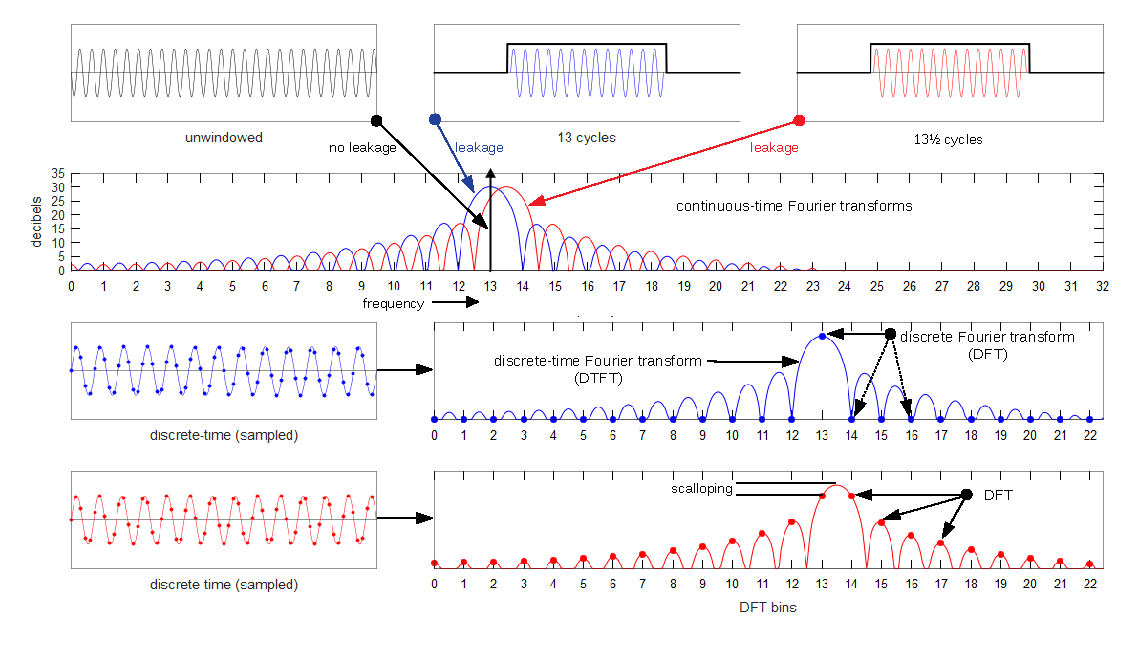
\includegraphics[scale=0.8]{papers/autotune/sections/fft/images/windows/Spectral.pdf}
	\caption{Darstellung der Fensterung und dessen mögliche Frequenzverschmierung/Unschärfe}\cite{wikipedia:Window}
	\label{fig:Spectral}
\end{figure}%

Zuerst wird das Signal $x(t)$ zeitkontinuierlich berachtet. Im ersten Beispiel in \ref{fig:Spectral} wird das unendliche, kontinuierliche Signal $x(t)$ schwarz im Frequenzbereich abgebildet. Man bildet dafür die Fourierreihe von $x(t)$. Als Resultat erhält man nur eine Frequenz. Diese ist durch einen schwarzen Pfeil dargestellt.\\

Beim zweiten Beispiel in \ref{fig:Spectral} (in Blau) wird das Signal $x(t)$ mit der Rechteck-Fensterfunktion $w_{1}(t)$ multipliziert. Auf das Resultat wird eine Fouriertransformation angewendet.\\
Wobei gilt: 
\begin{equation}
	w_{1}(t)= \left\{\begin{array}{lll}{0,} & {t<\alpha}  \\ {1,}&{\alpha\leq t \leq\beta_{1}} \\ {0,} &{t>\beta_{1}}\end{array}\right\}
\end{equation}
\begin{equation}
	\hat{x_{1}}(\omega)=\frac{1}{\sqrt{2 \pi}} \int_{-\infty}^{\infty} w_{1}(t)\cdot x(t) \cdot e^{-i \omega t} \,dt
\end{equation}

Dabei decken $\alpha$ und $\beta_{1}$ ein Zeitintervall von $13$ Perioden ab. Im Frequenzbereich ist nun in blau ersichtlich, dass die Fourier-Transformation eine deutliche Unschärfe zur Folge hat. Diese Unschärfe ist im kontinuierlichen Spektrum ersichtlich. Das Maxima der Fouriertransformierten korreliert jedoch mit dem einen Resultat des originalen Signales $x(t)$\\




Im letzten Fall in \ref{fig:Spectral} wird $x(t)$ mit der etwas längeren Rechteck-Fensterfunktion $w_{2}(t)$ multipliziert.\\
Wobei gilt: 
\begin{equation}
	w_{2}(t)= \left\{\begin{array}{lll}{0,}&{t<\alpha}  \\ {1,}&{\alpha\leq t \leq\beta_{2}}  {1}\\ {0,}&{t>\beta_{2}}\end{array}\right\}
\end{equation}
\begin{equation}
	\hat{x_{2}}(\omega)=\frac{1}{\sqrt{2 \pi}} \int_{-\infty}^{\infty} w_{2}(t)\cdot x(t) \cdot e^{-i \omega t} \,dt
\end{equation}

Wobei $\alpha$ und $\beta_{2}$ ein Zeitintervall von $13\frac{1}{2}$ Perioden abdecken. Nun sieht man nicht nur eine Unschärfe, sondern auch eine fehlende Korrelation zwischen dem Maxima der Fouriertansformierten und der eigentlichen Frequenz des Signales $x(t)$.\\

Betrachtet man nun die diskrete Fouriertransformierte der beiden gefensterten Signale, kann man Folgendes erkennen: Ist das Signal genau über ein Vielfaches der Periode gefenstert, kann man im diskreten Fall keine Frequenzunschärfe erkennen. Trifft die Fensterung jedoch auf eine zufällige Stelle im Signal und deckt nicht gerade eine Periode ab, zeigen die diskrete Werte ein nur schwer zu interpretierendes Ergebnis an. Man spricht von einer Unschärfe im Frequenzbereich. Durch die Unschärfe werden nicht nur die eigentlichen Frequenzen des Signales $x(t)$ abgebildet. Stattdessen werden die Frequenzen über ein ganzes Band verschmiert.\\

Möchte man nun ein reales Signal analysieren kommt es zu einem ähndlichen verhalten. Reale Signale, die meistens nicht periodisch auftreten und mit diskreten Werten beschrieben sind, werden solche Unschärfen aufzeigen. Nun gibt es verschiedenste Methoden um eine Frequenzanalyse zu realisieren. In diesem Paper wird jedoch nur auf die STFT und die Wavelet-Transformation eingegangen. 


\subsection{Zeitkontinuierliche STFT}

Das Produkt des Signals $x(t)$ mit der Fensterfunktion $w(t) $ liefert uns also eine neue Funktion die im Bereich ausserhalb des Fensters alle Werte auf null gesetzt hat. In der Anwendung sind diese Fenster meistens ein wenig überlappend damit kein Datenverlust entsteht. \\
Die verallgemeinerte zeitkontiunierliche STFT ist  gegeben als:
\begin{equation}
	\hat{f}(\tau, \omega)=\int_{-\infty}^{\infty} f(t)\cdot w(t-\tau)\cdot e^{-i \omega t} dt
\end{equation}
mit der Kreisfrequenz  $\omega $

\subsection{Zeitdiskrete STFT}
Bei der zeitdiskreten STFT liegt das Signal in einzelnen Abtastwerten vor. Diese Abtastwerte werden dann durch die Fensterfunktionen in einzelne Abschnitte unterteilt. \\
Die diskrete STFT ist gegeben als:
\begin{equation}
	\hat{f}(m, \omega)=\sum_{n=-\infty}^{\infty} f_{n} \cdot w_{n-m}\cdot e^{-i \omega n}
\end{equation}


\subsection{Fensterfunktionen}
Um die Unschärfeproblematik der STFT zu verbessern, gibt es eine ganze Reihe an verschiedenen Fensterfunktionen die verwendet werden können, um ein besseres Resultat zu erreichen. Die Auswahl der Funktion ist dabei anwendungsspezifisch. In der Folgenden Tabelle \ref{fig:STFTtab} findet man eine kleine Auswahl mit dem jeweiligen verhalten im Frequenzbereich. 


\begin{figure}[!ht]
	\begin{minipage}{.4\columnwidth}
		\textbf{Rechteck-Fenster}\\
		$w_{n}=1$
	\end{minipage}%
	\begin{minipage}{.6\columnwidth}
		\centering
		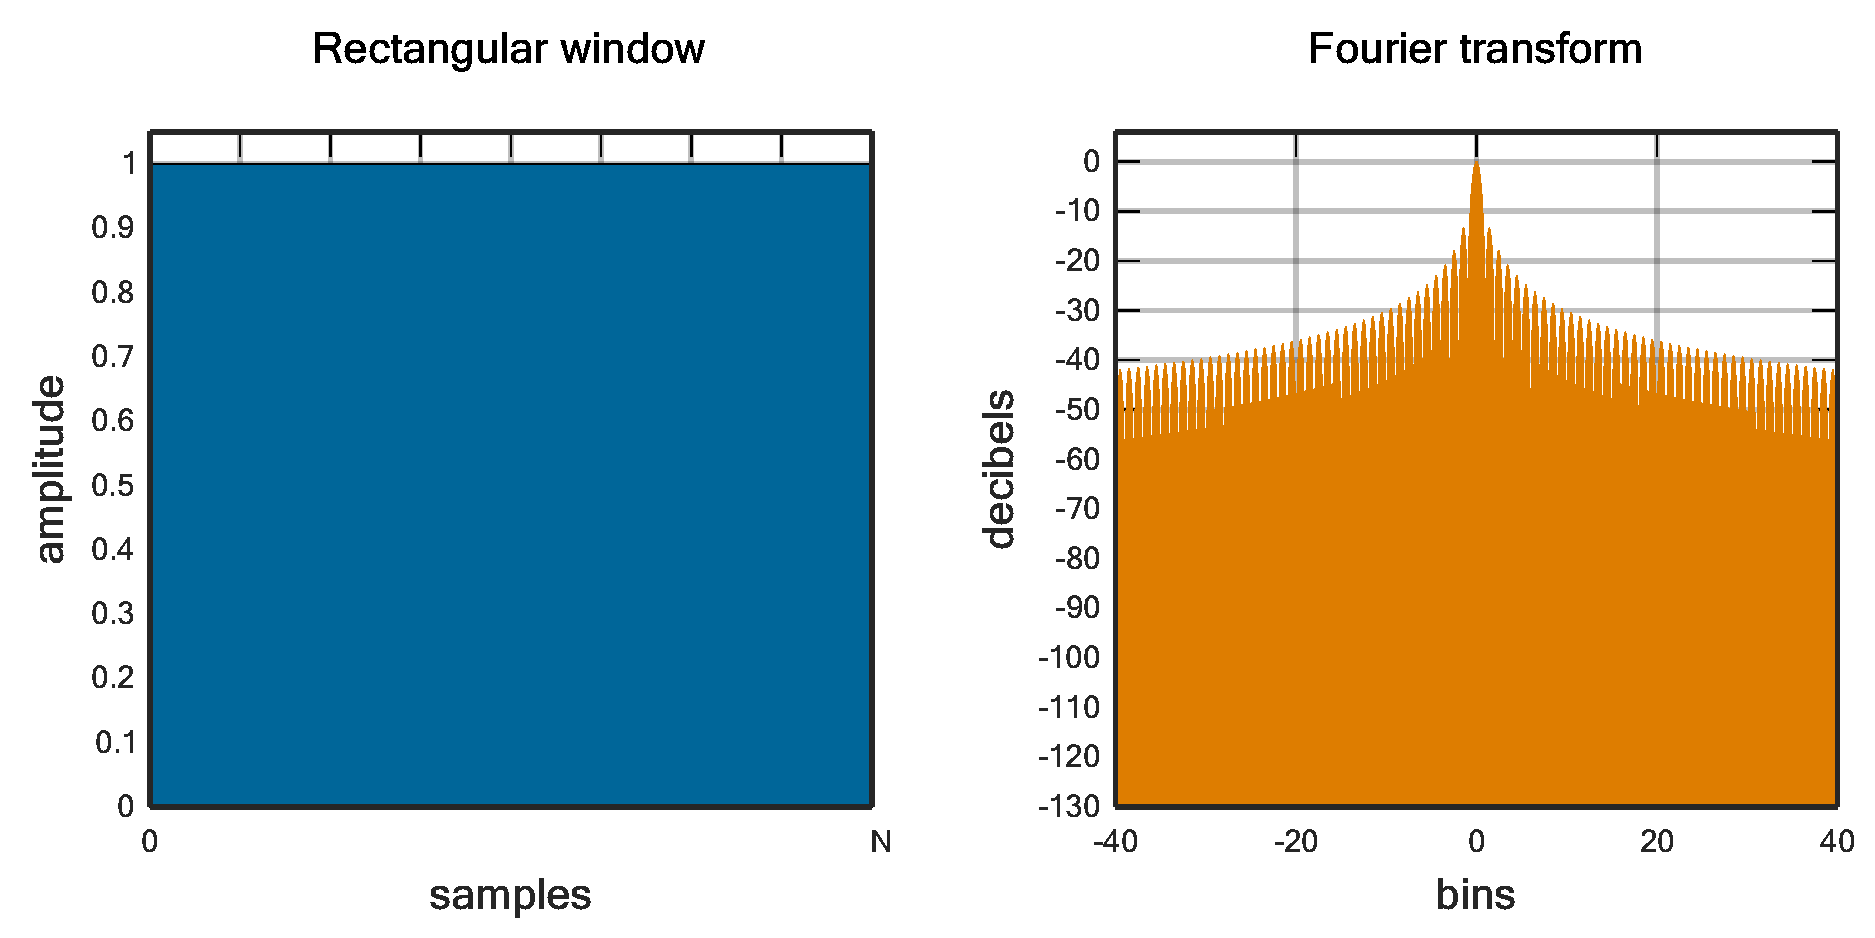
\includegraphics[width=\linewidth]{papers/autotune/sections/fft/images/windows/Rectangular.pdf}
	\end{minipage}


	\begin{minipage}{.4\columnwidth}
		\textbf{Gauss-Fenster} mit $\sigma = 0.4$\\
		$w_{n}=e^{-\frac{1}{2}\left(\frac{n-N / 2}{\sigma N / 2}\right)^{2}},$\\
		$ \quad 0 \leq n \leq N$\\
		$\sigma \leq 0.5$
	\end{minipage}%
	\begin{minipage}{.6\columnwidth}
		\centering
		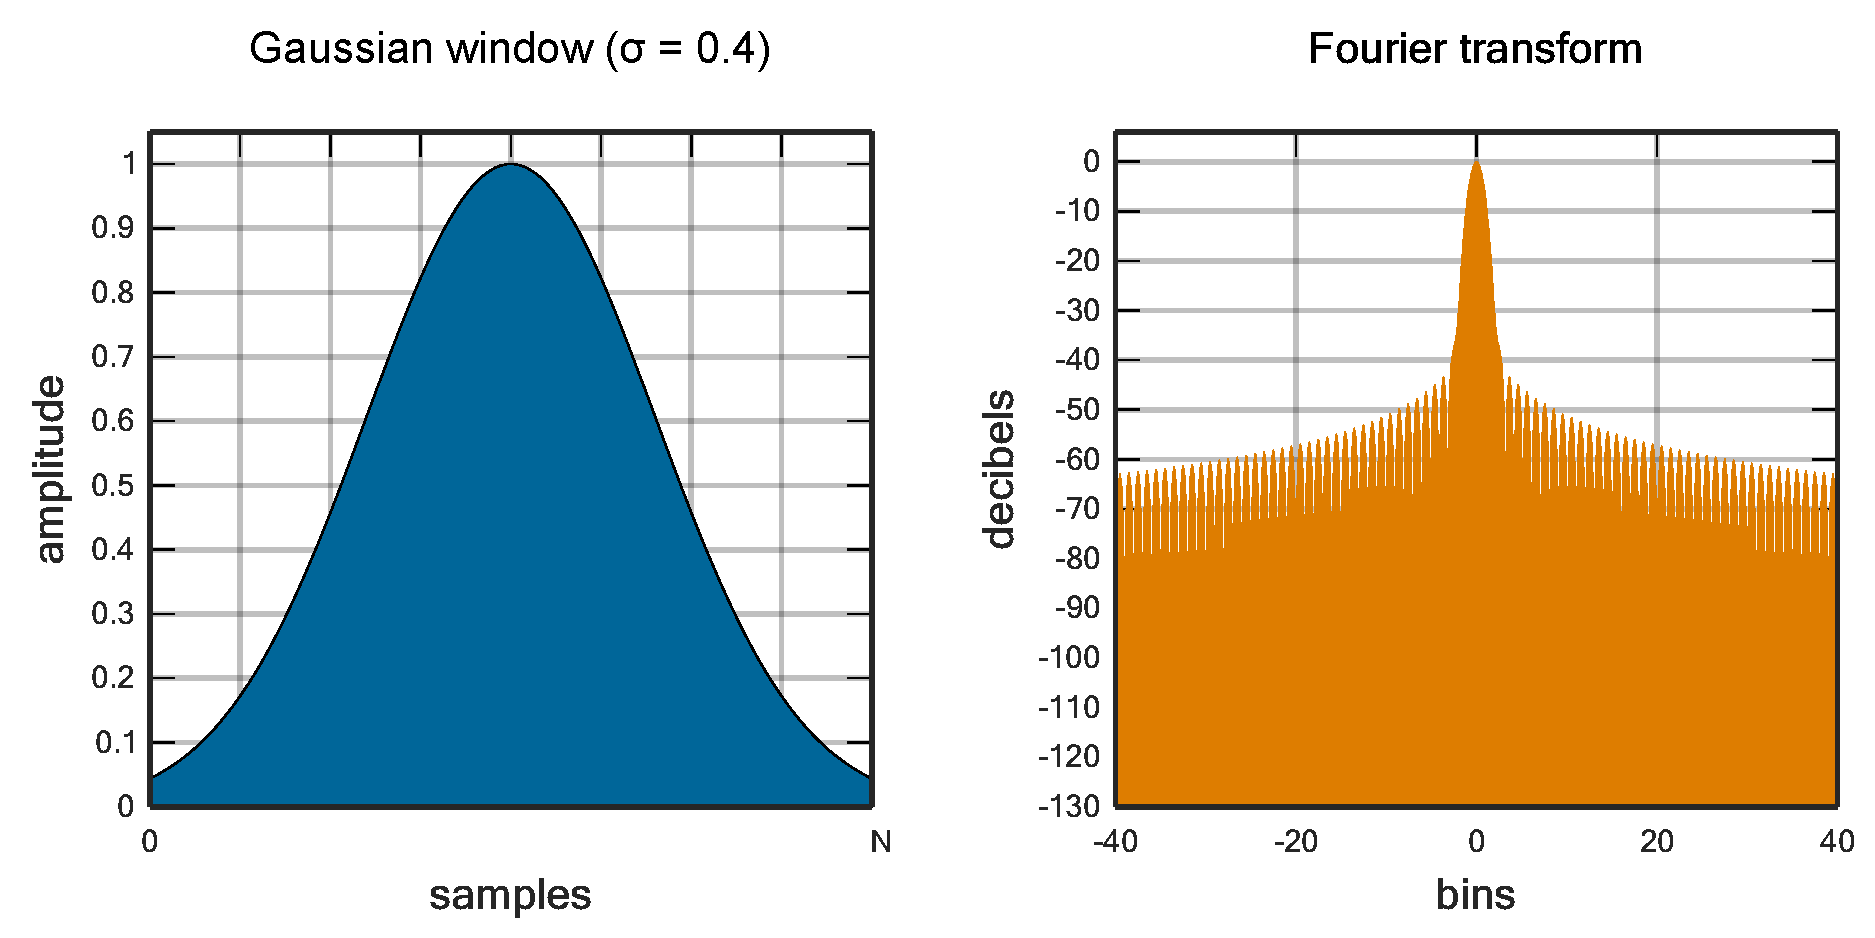
\includegraphics[width=\linewidth]{papers/autotune/sections/fft/images/windows/Gauss.pdf}
	\end{minipage}


	\begin{minipage}{.4\columnwidth}
		\textbf{Blackman-Fenster}\\
		$\begin{array}{l}{w_{n}=a_{0}-a_{1} \cos \left(\frac{2 \pi n}{N}\right)+a_{2} \cos \left(\frac{4 \pi n}{N}\right)} \\ 		{a_{0}=\frac{1-\alpha}{2} ; \quad a_{1}=\frac{1}{2} ; \quad a_{2}=\frac{\alpha}{2}}\end{array}$
	\end{minipage}%
	\begin{minipage}{.6\columnwidth}
		\centering
		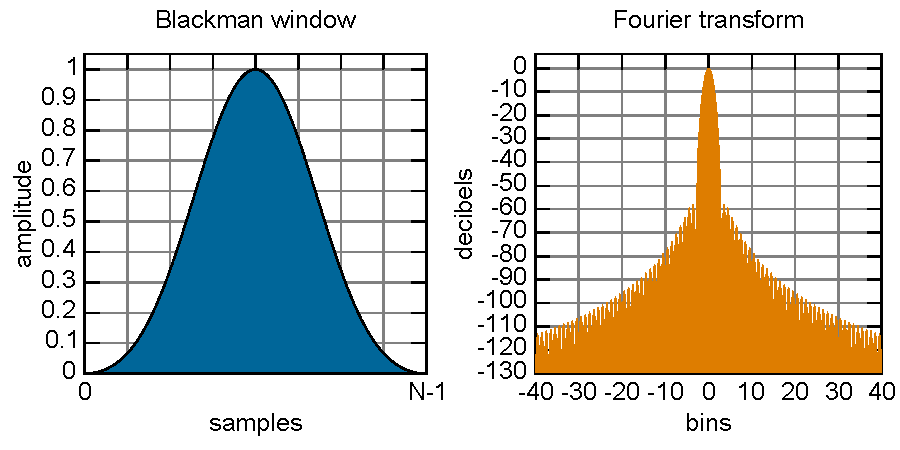
\includegraphics[width=\linewidth]{papers/autotune/sections/fft/images/windows/Blackman.pdf}
	\end{minipage}


	\begin{minipage}{.4\columnwidth}
		\textbf{Blackman-Harris-Fenster}\\
		$w_{n}=a_{0}-a_{1} \cos \left(\frac{2 \pi n}{N}\right)+a_{2} \cos \left(\frac{4 \pi n}{N}\right)-a_{3} \cos \left(\frac{6 \pi n}{N}\right)$\\
		wobei:
		$a_{0}=0.35875 ; \quad a_{1}=0.48829 ;$\\
		$ \quad a_{2}=0.14128 ; \quad a_{3}=0.01168$
	\end{minipage}%
	\begin{minipage}{.6\columnwidth}
		\centering
		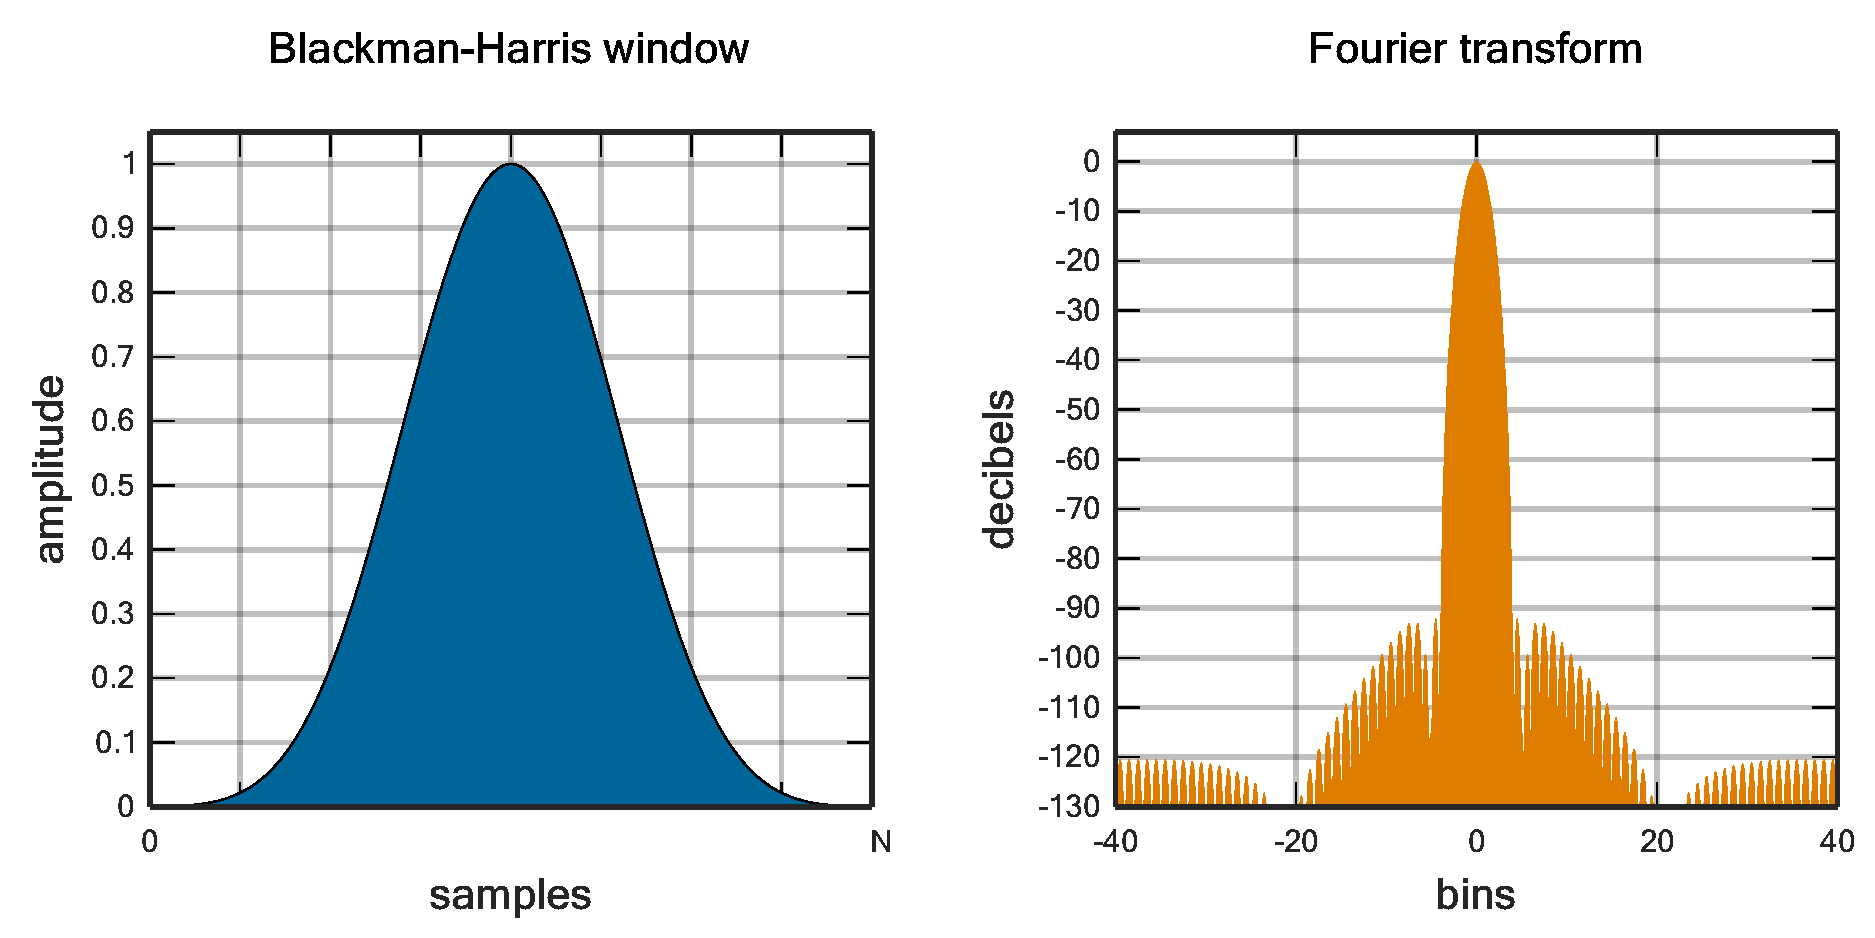
\includegraphics[width=\linewidth]{papers/autotune/sections/fft/images/windows/Blackman-Harris.pdf}
	\end{minipage}

\caption{Verschiedene Fensterfunktionen und deren Beschreibung}\cite{wikipedia:Window}
\label{fig:STFTtab}
\end{figure}
\newpage


\subsection{Verhalten der STFT}

Wenn man ein Signal mit einer Fensterfunktion analysiert, zerteilt man es vertikal in der Zeitachse. Diese vertikalen Streifen besitzen die Breite eines Fensterintervalles. Wendet man nun darauf die Fourier-Transformation an, wird jeder dieser Streifen zu Rechtecken im Spektrum aufgeteilt. Die jeweilige Höhe dieser Rechtecke wird durch die Unschärferelation bestimmt. Daraus folgt, dass es bei einem breiteren Streifen eine besser Frequenzauflösung ergibt, was jedoch eine schlechtere Zeitauflösung bedeutet. In der Abbildung \ref{fig:stftauf} kann man die grafische Darstellung der Zeit-Frequenz-Auflösung der STFT sehen. Bei gleichbleibendem Flächeninhalt der einzelnen Rechtecke, ist auf der linken Seite eine feinere Zeitauflösung zu sehen. Der Graph rechts weist dabei eine bessere Frequenzauflösung auf. \\

Dies kann mit der Küpfmüllerschen Unbestimmtheitsrelation begründet werden. Sie besagt, dass die Zeitdauer $\delta t$ und die Bandbreite $\delta f$ eines Signals nicht beliebig klein werden können.  
\[\Delta t \cdot \Delta f \geq q\]
$q$ kann dabei je nach Defintion der Zeitdauer und Bandbreite den Wert 0.5 oder 1 annehmen. Eine zur Heisenbergschen Unschärferelation analoge Aussage, welche auf die Nachrichtentechnik übernommen werden kann.


\begin{figure}[!ht]
	\centering
	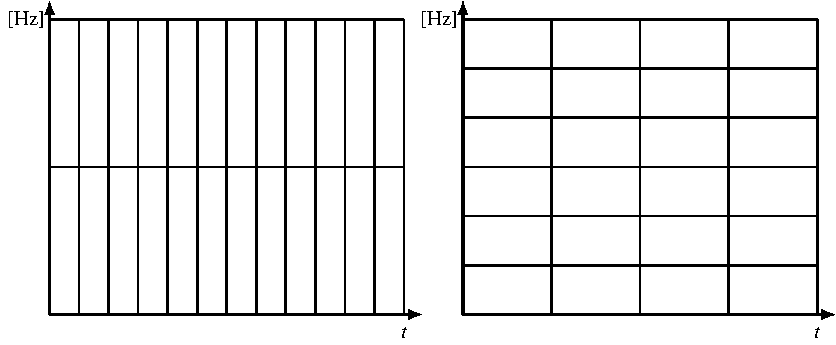
\includegraphics[width=0.7\linewidth]{papers/autotune/sections/fft/images/windows.pdf}
	\caption{STFT Zeit-Frequenz-Auflösung}\label{fig:stftauf}	
\end{figure}




Um die Unschärferelation zu veranschaulichen wird ein Signal generiert und STFT analysiert. Die STFT wird dafür mehrmals mit verschiedenen Fensterlängen auf das selbe Signal angewendet. So können die verschiedenen Fensterlängen und deren STFT Resultate verglichen werden. Beim generierten Signal handelt es sich um einen modulierten Frequensweep der von 0 bis 400\text{[Hz]} reicht. Die Definition der verwendeten Frequenzsweepes $x_{\text{sweep}}(t)$ ist folgendermassen:

\begin{equation}
x_{sweep}(t)=\sin \left(2 \pi \int_{0}^{t} f(\tau) \mathrm{d} \tau\right)=\sin \left(2 \pi \int_{0}^{t}\left(f_{0}+k \tau\right) \mathrm{d} \tau\right)=\sin \left(2 \pi\left(f_{0}+\frac{k}{2} t\right) t\right)
\end{equation} 

Der Sweep wird nun mit einem viel langsameren Cosinus moduliert. Die Defenition des zu analysierende Signales $f(t)$ lautet dementsprechend:
\begin{equation}
f(t)= (-0.5\cdot \cos(nt)+0.5)\cdot x(t)=(-0.5\cdot \cos(nt)+0.5)\cdot \sin \left(2 \pi \int_{0}^{t} f(\tau) \mathrm{d} \tau\right)
\end{equation} \label{eq:sin-sweep}
Bei $n$ handelt es sich um die Anzahl von Perioden des Cosinus in einer Zeit von $2\pi$\\
Die Funktion $f(t)$  wird dann mit dem STFT Verfahren analysiert. Insgesamt wurde $f(t)$ von vier verschiedenen Fensterfunktionen analysiert. Jede Analyse wurde mit der Blackman Fensterfunktion durchgeführt. Die Veränderung der Fensterlänge trägt zu dem Verständnis der Unschärferelation bei. Die Definition der verwendete Blackman-Fensterfunktion kann in der Tabelle \ref{fig:STFTtab} gefunden werden.\\


In der Grafik \ref{fig:STFT} kann diese Unschärferelation beobachtet werden. Die Unschärfe wird jetzt gut erkennbar, da man ein beliebiges Signal mit zeitlich verschieden langen Fenstern Analysiert. Dabei sollte bei diskreten Funktionen dies direkt in anzahl Samples pro Fenster gesehen werden muss.\\



\begin{figure}[!ht]
	\centering
	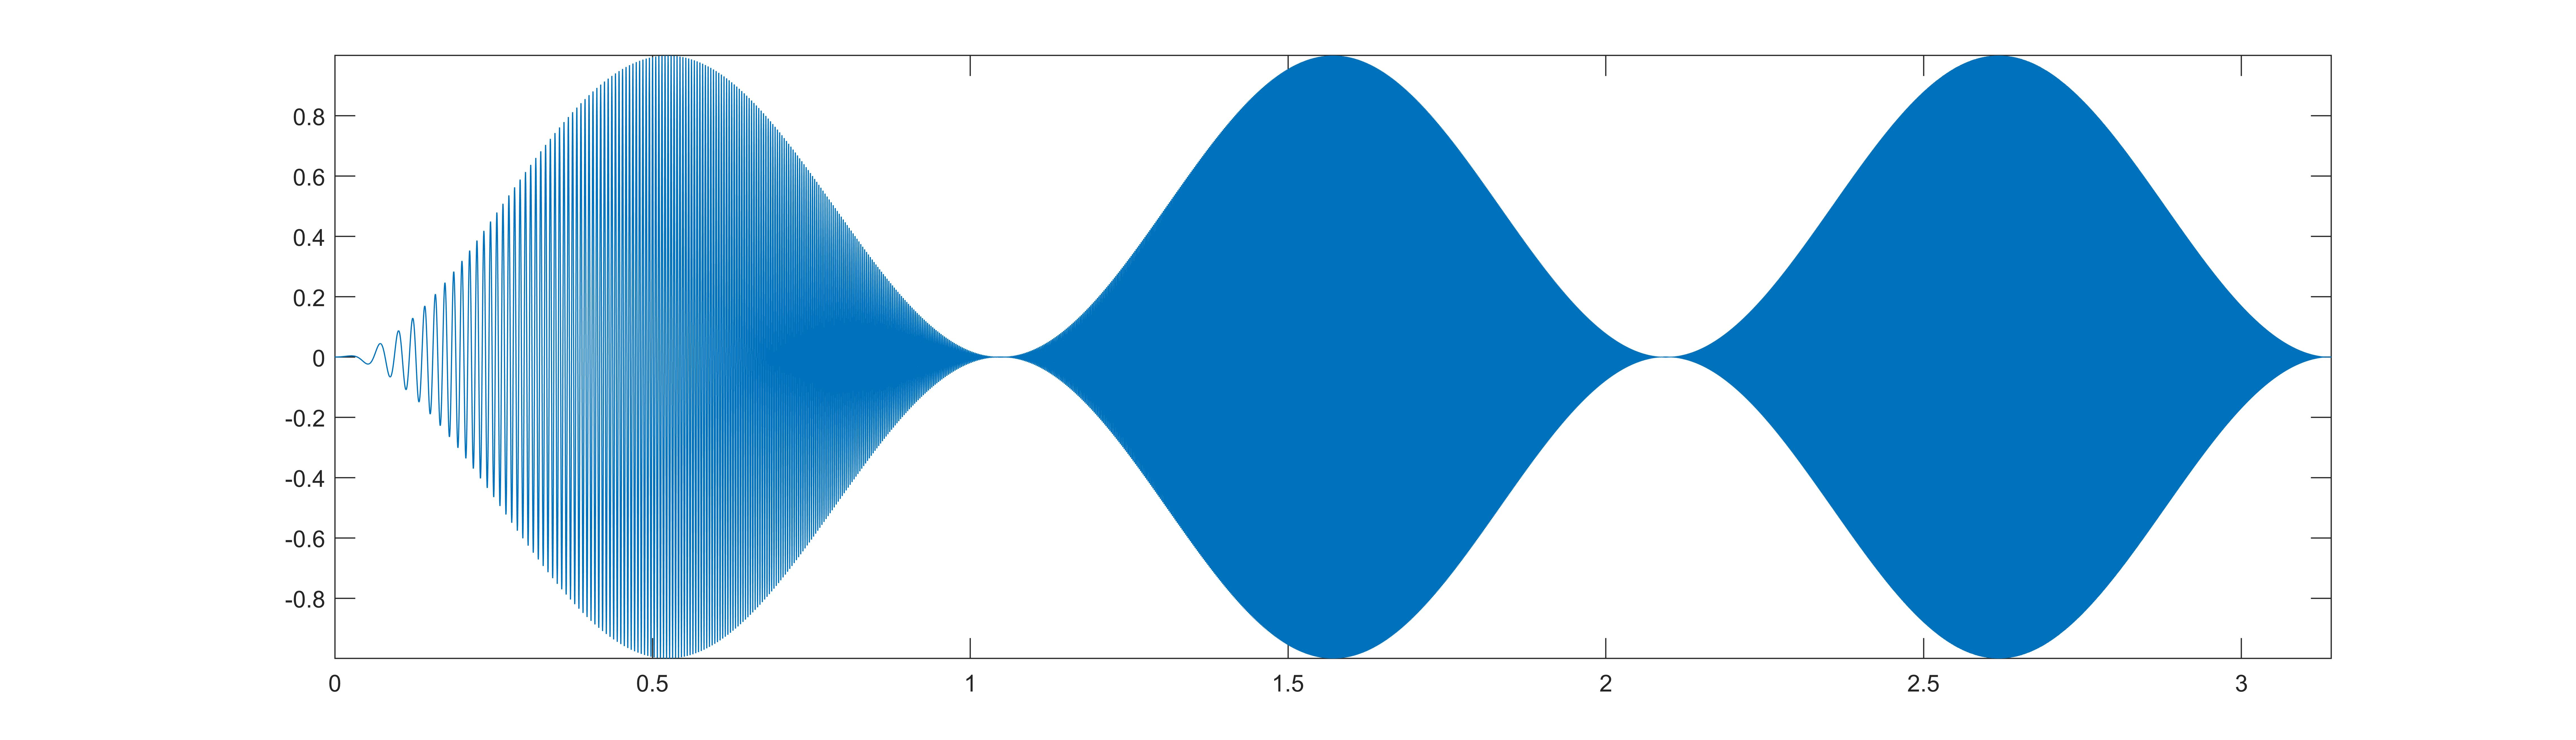
\includegraphics[width=\linewidth]{papers/autotune/sections/fft/signal.jpg}
	\captionof{figure}{Sweep Signal 0-400$Hz$}\label{fig:stftsig}
	\begin{tabularx}{\columnwidth}{XX}
		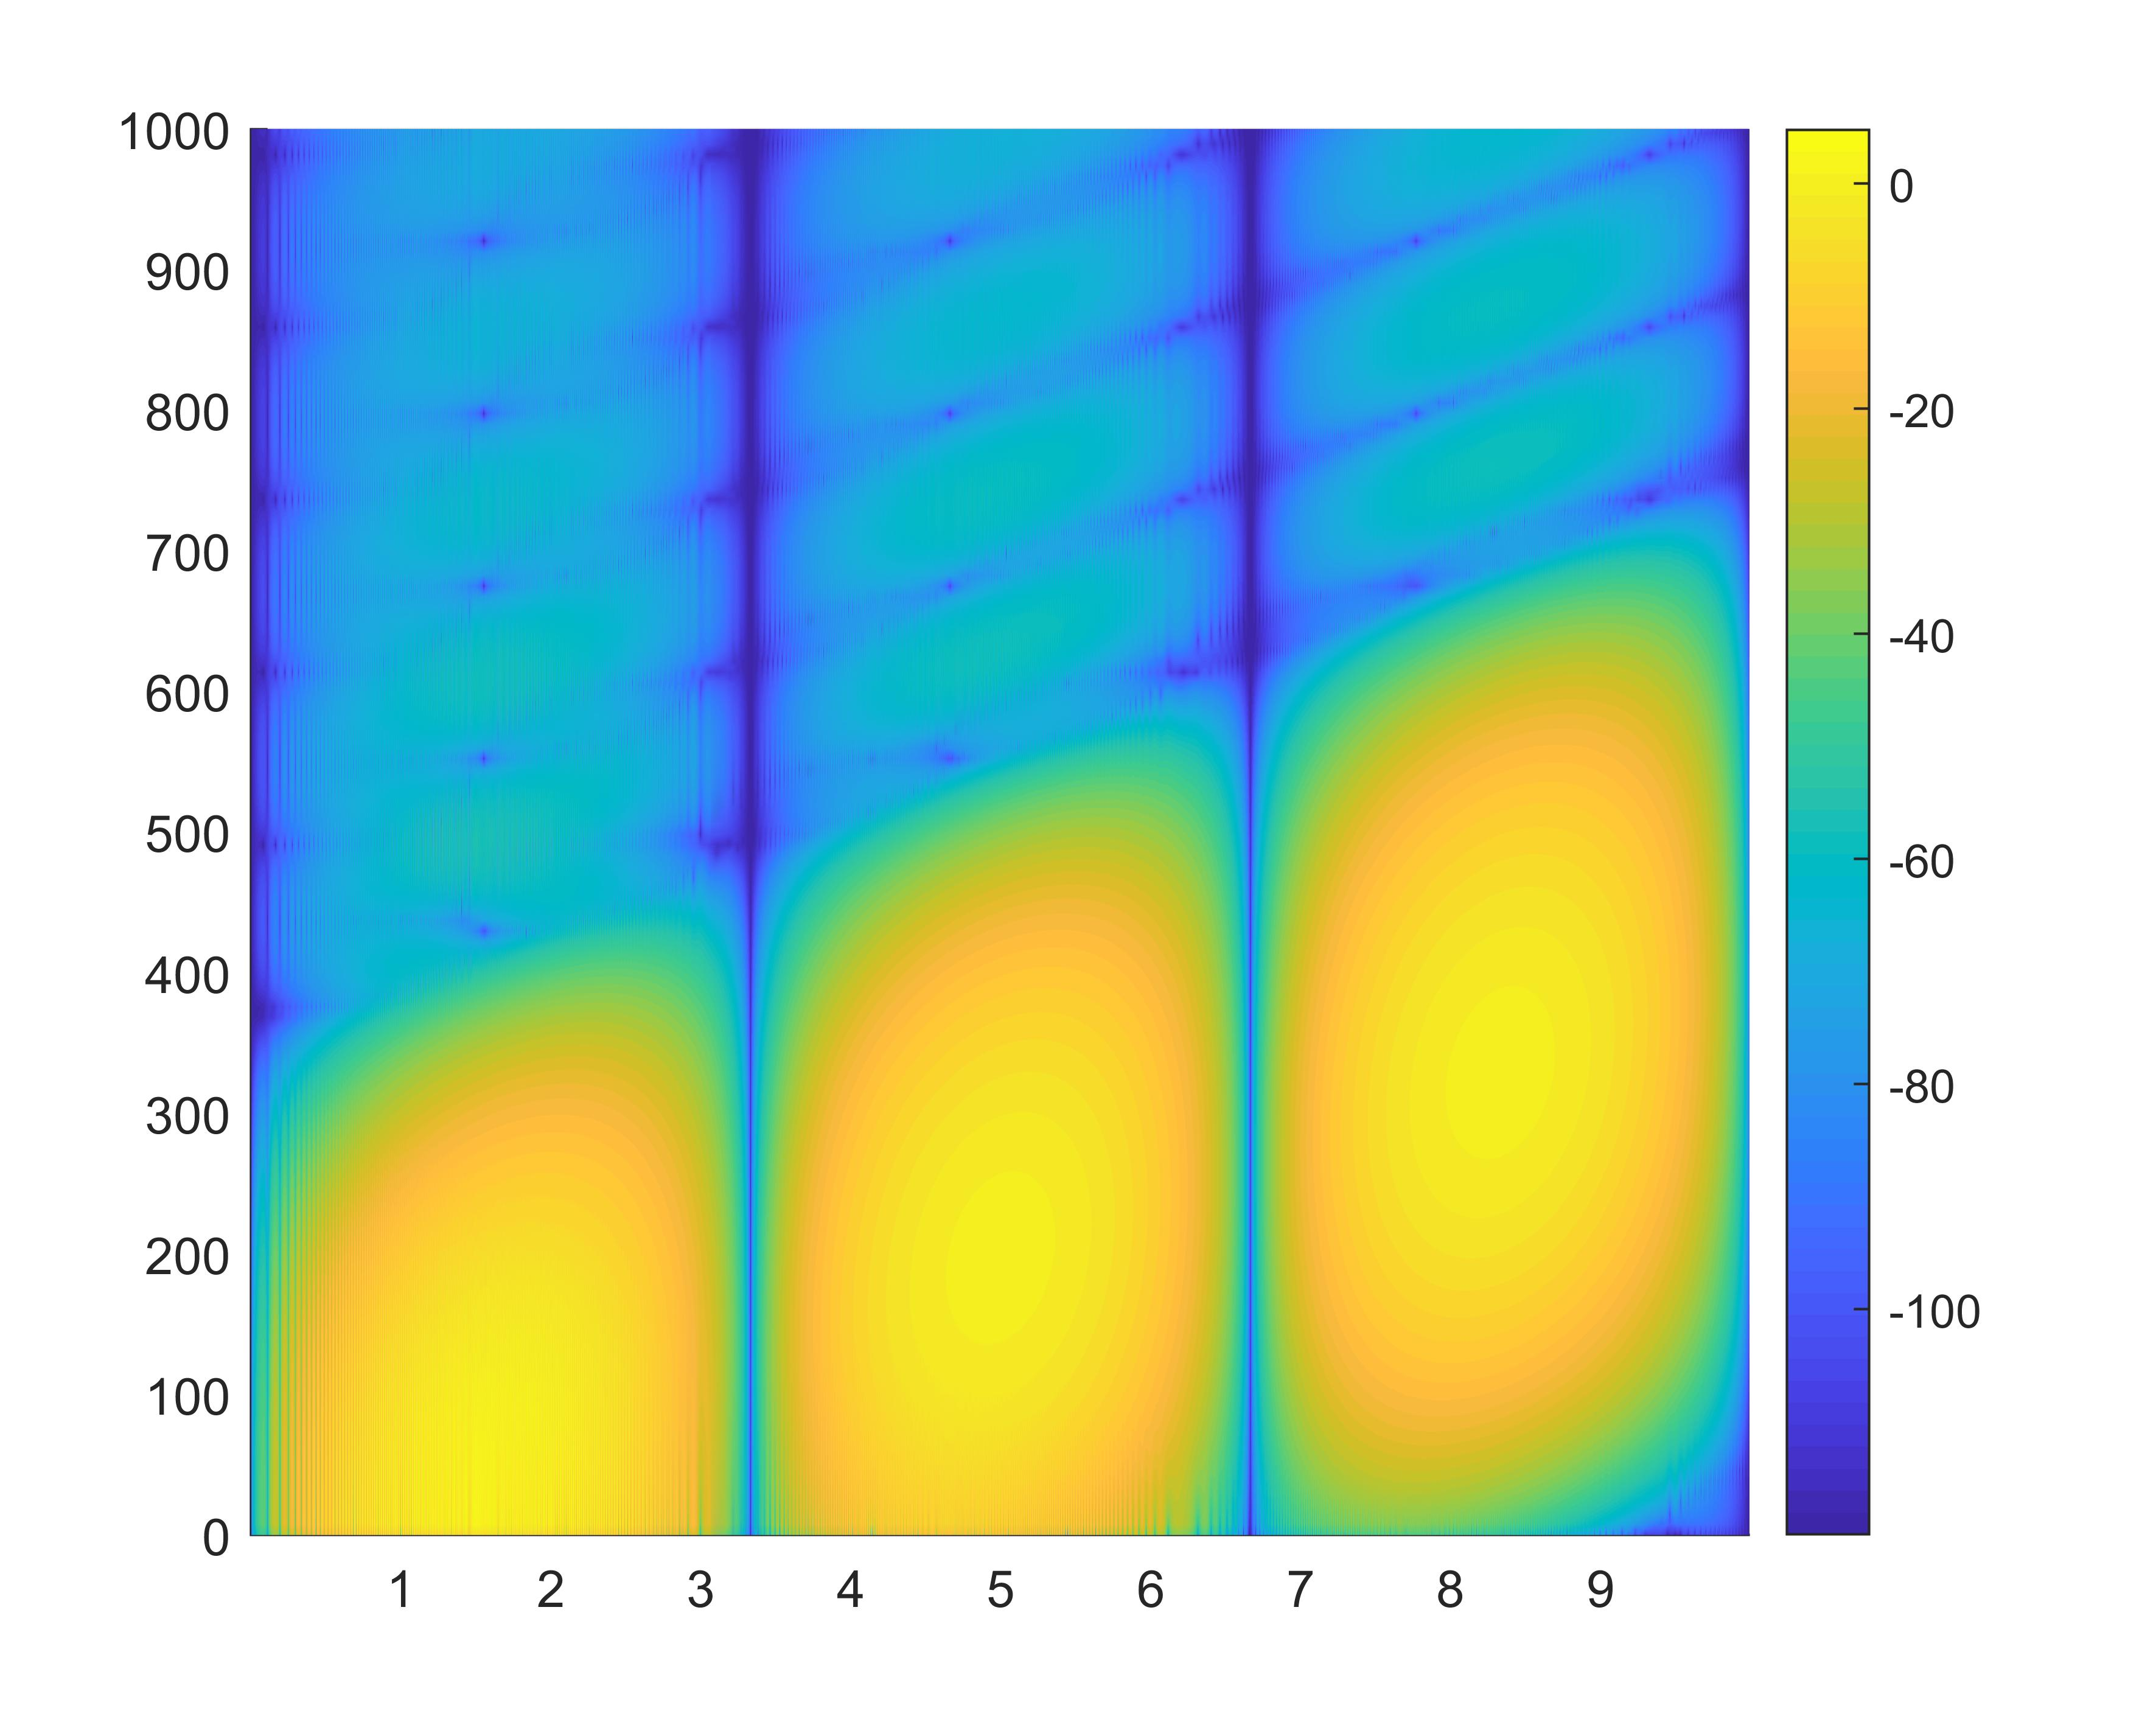
\includegraphics[width=\linewidth]{papers/autotune/sections/fft/stft256.jpg}
		\captionof{figure}{256 Sample Fenster}\label{fig:stft256}
		&   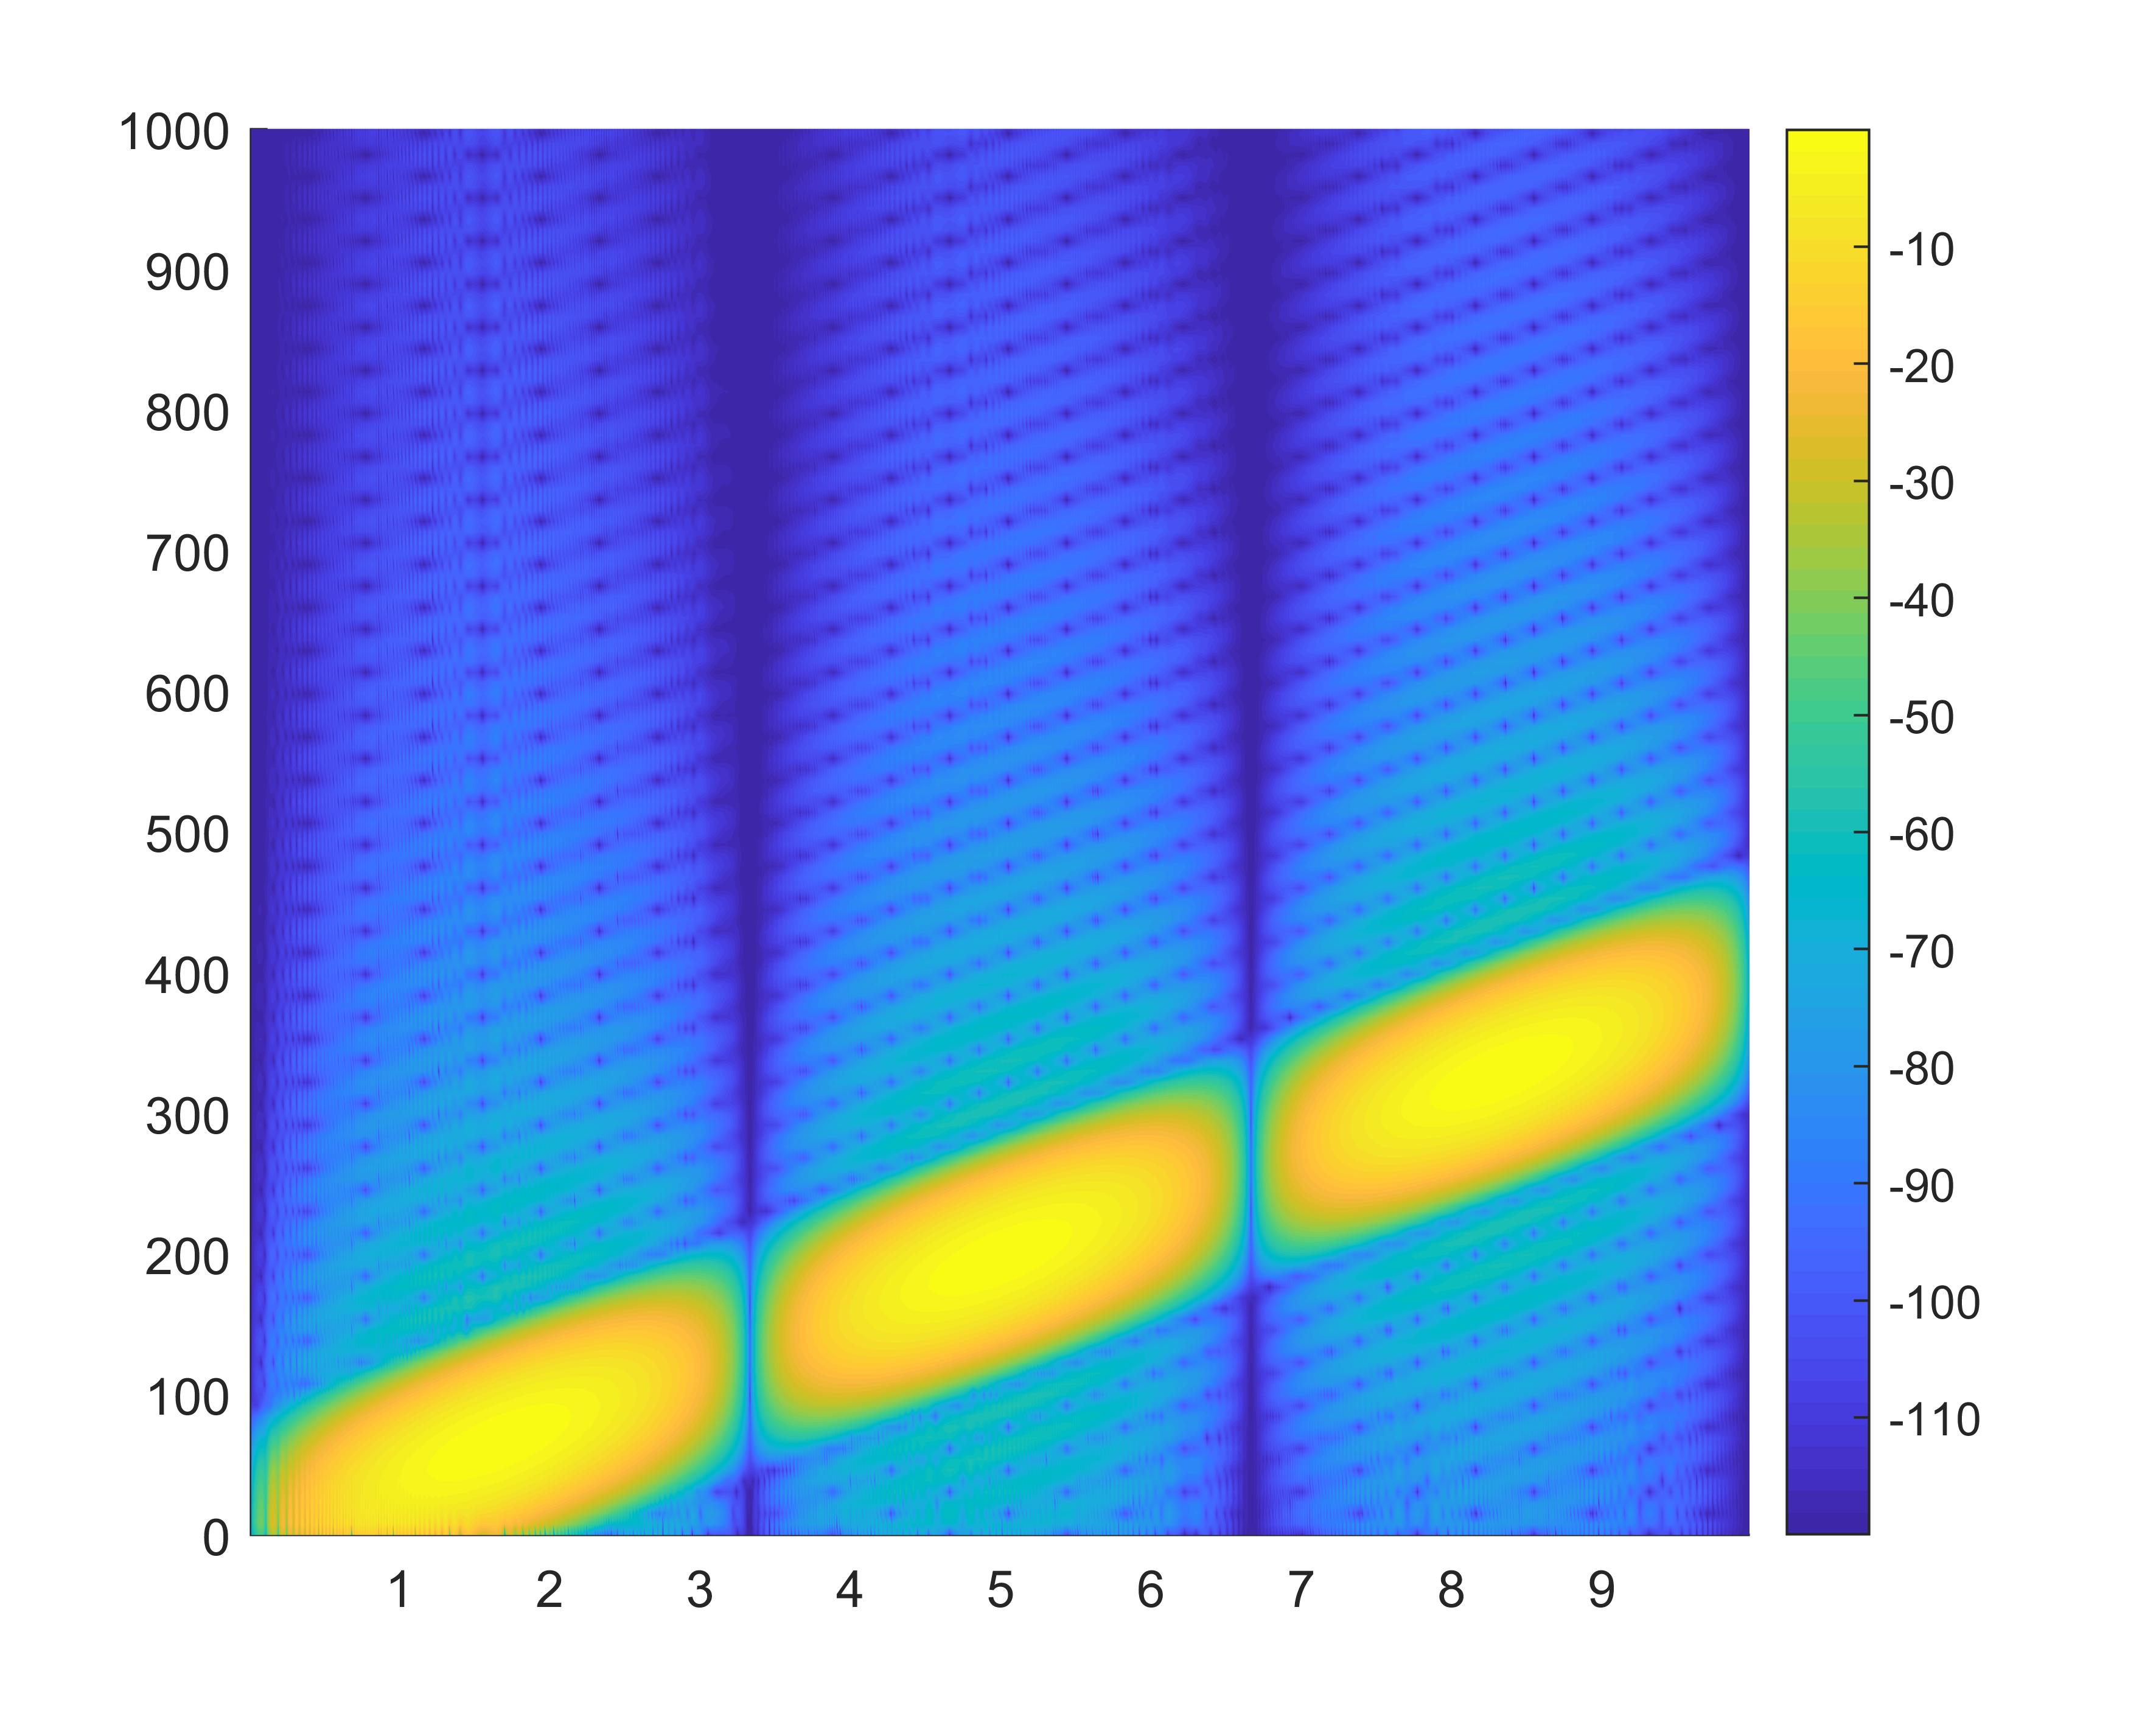
\includegraphics[width=\linewidth]{papers/autotune/sections/fft/stft1024.jpg}   
		\captionof{figure}{1024 Sample Fenster}\label{fig:stft1024}              \\    
		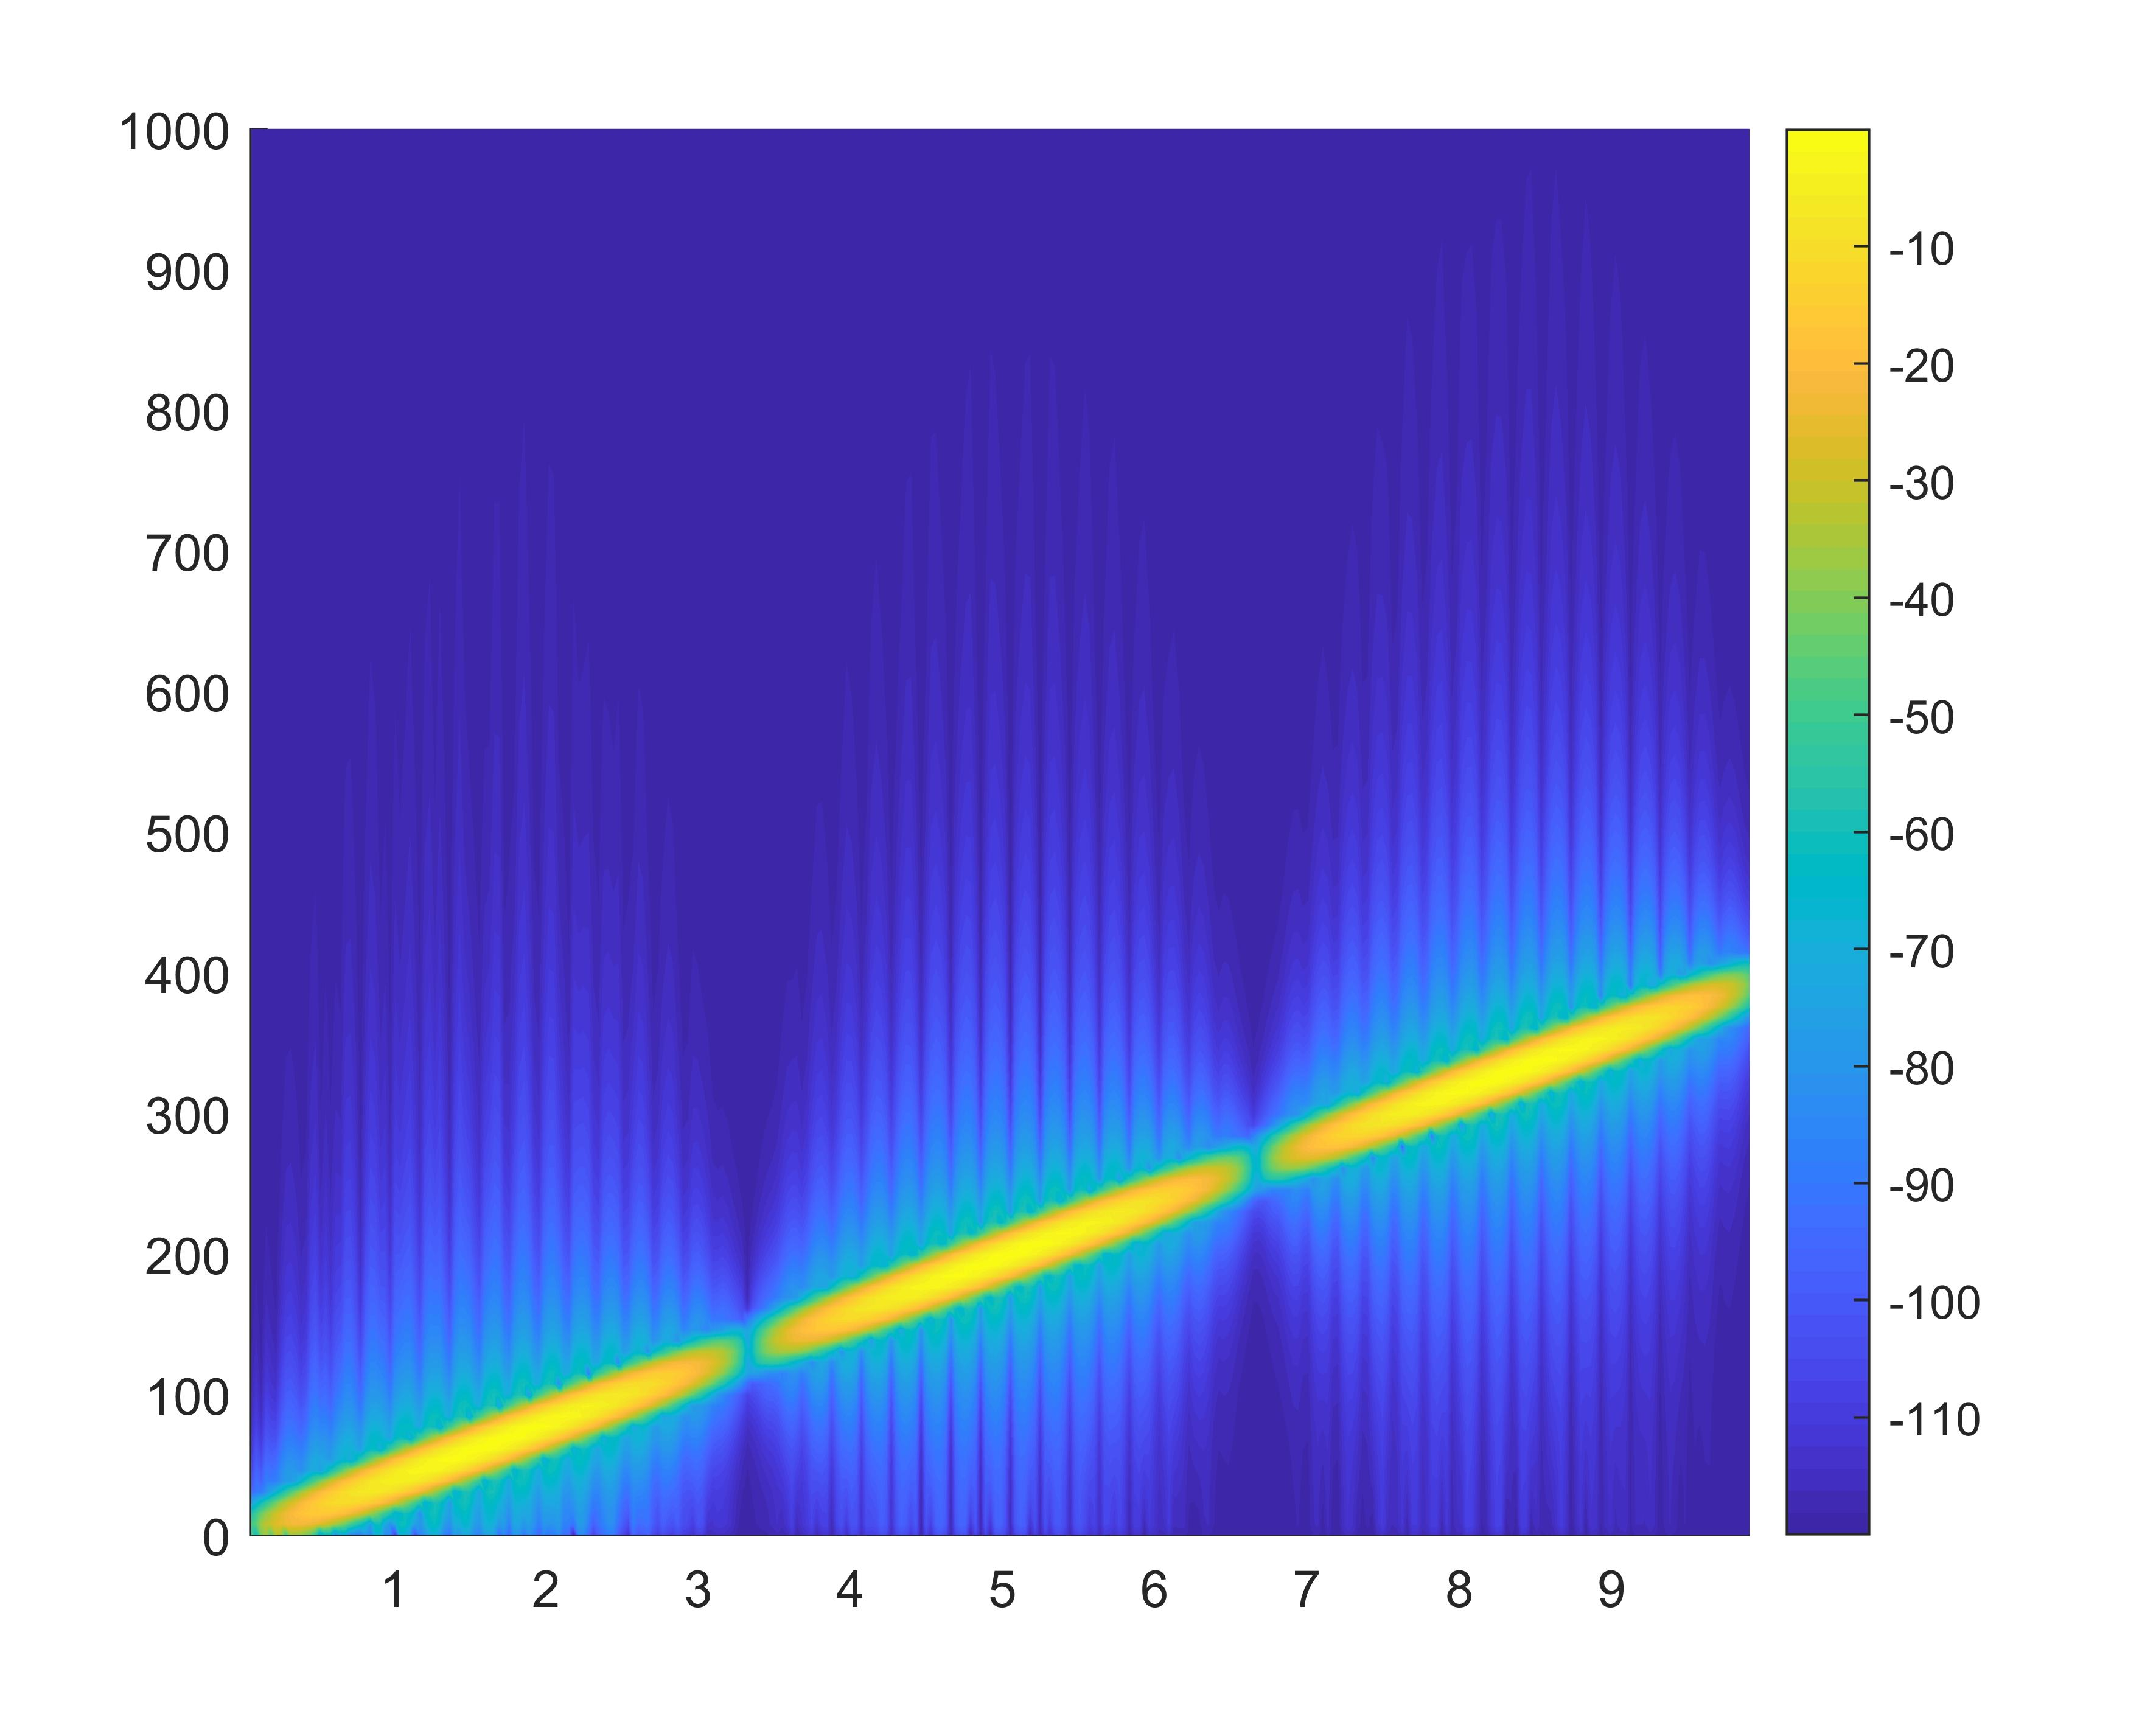
\includegraphics[width=\linewidth]{papers/autotune/sections/fft/stft4096.jpg}
		\captionof{figure}{4096 Sample Fenster}\label{fig:stft4096}
		&   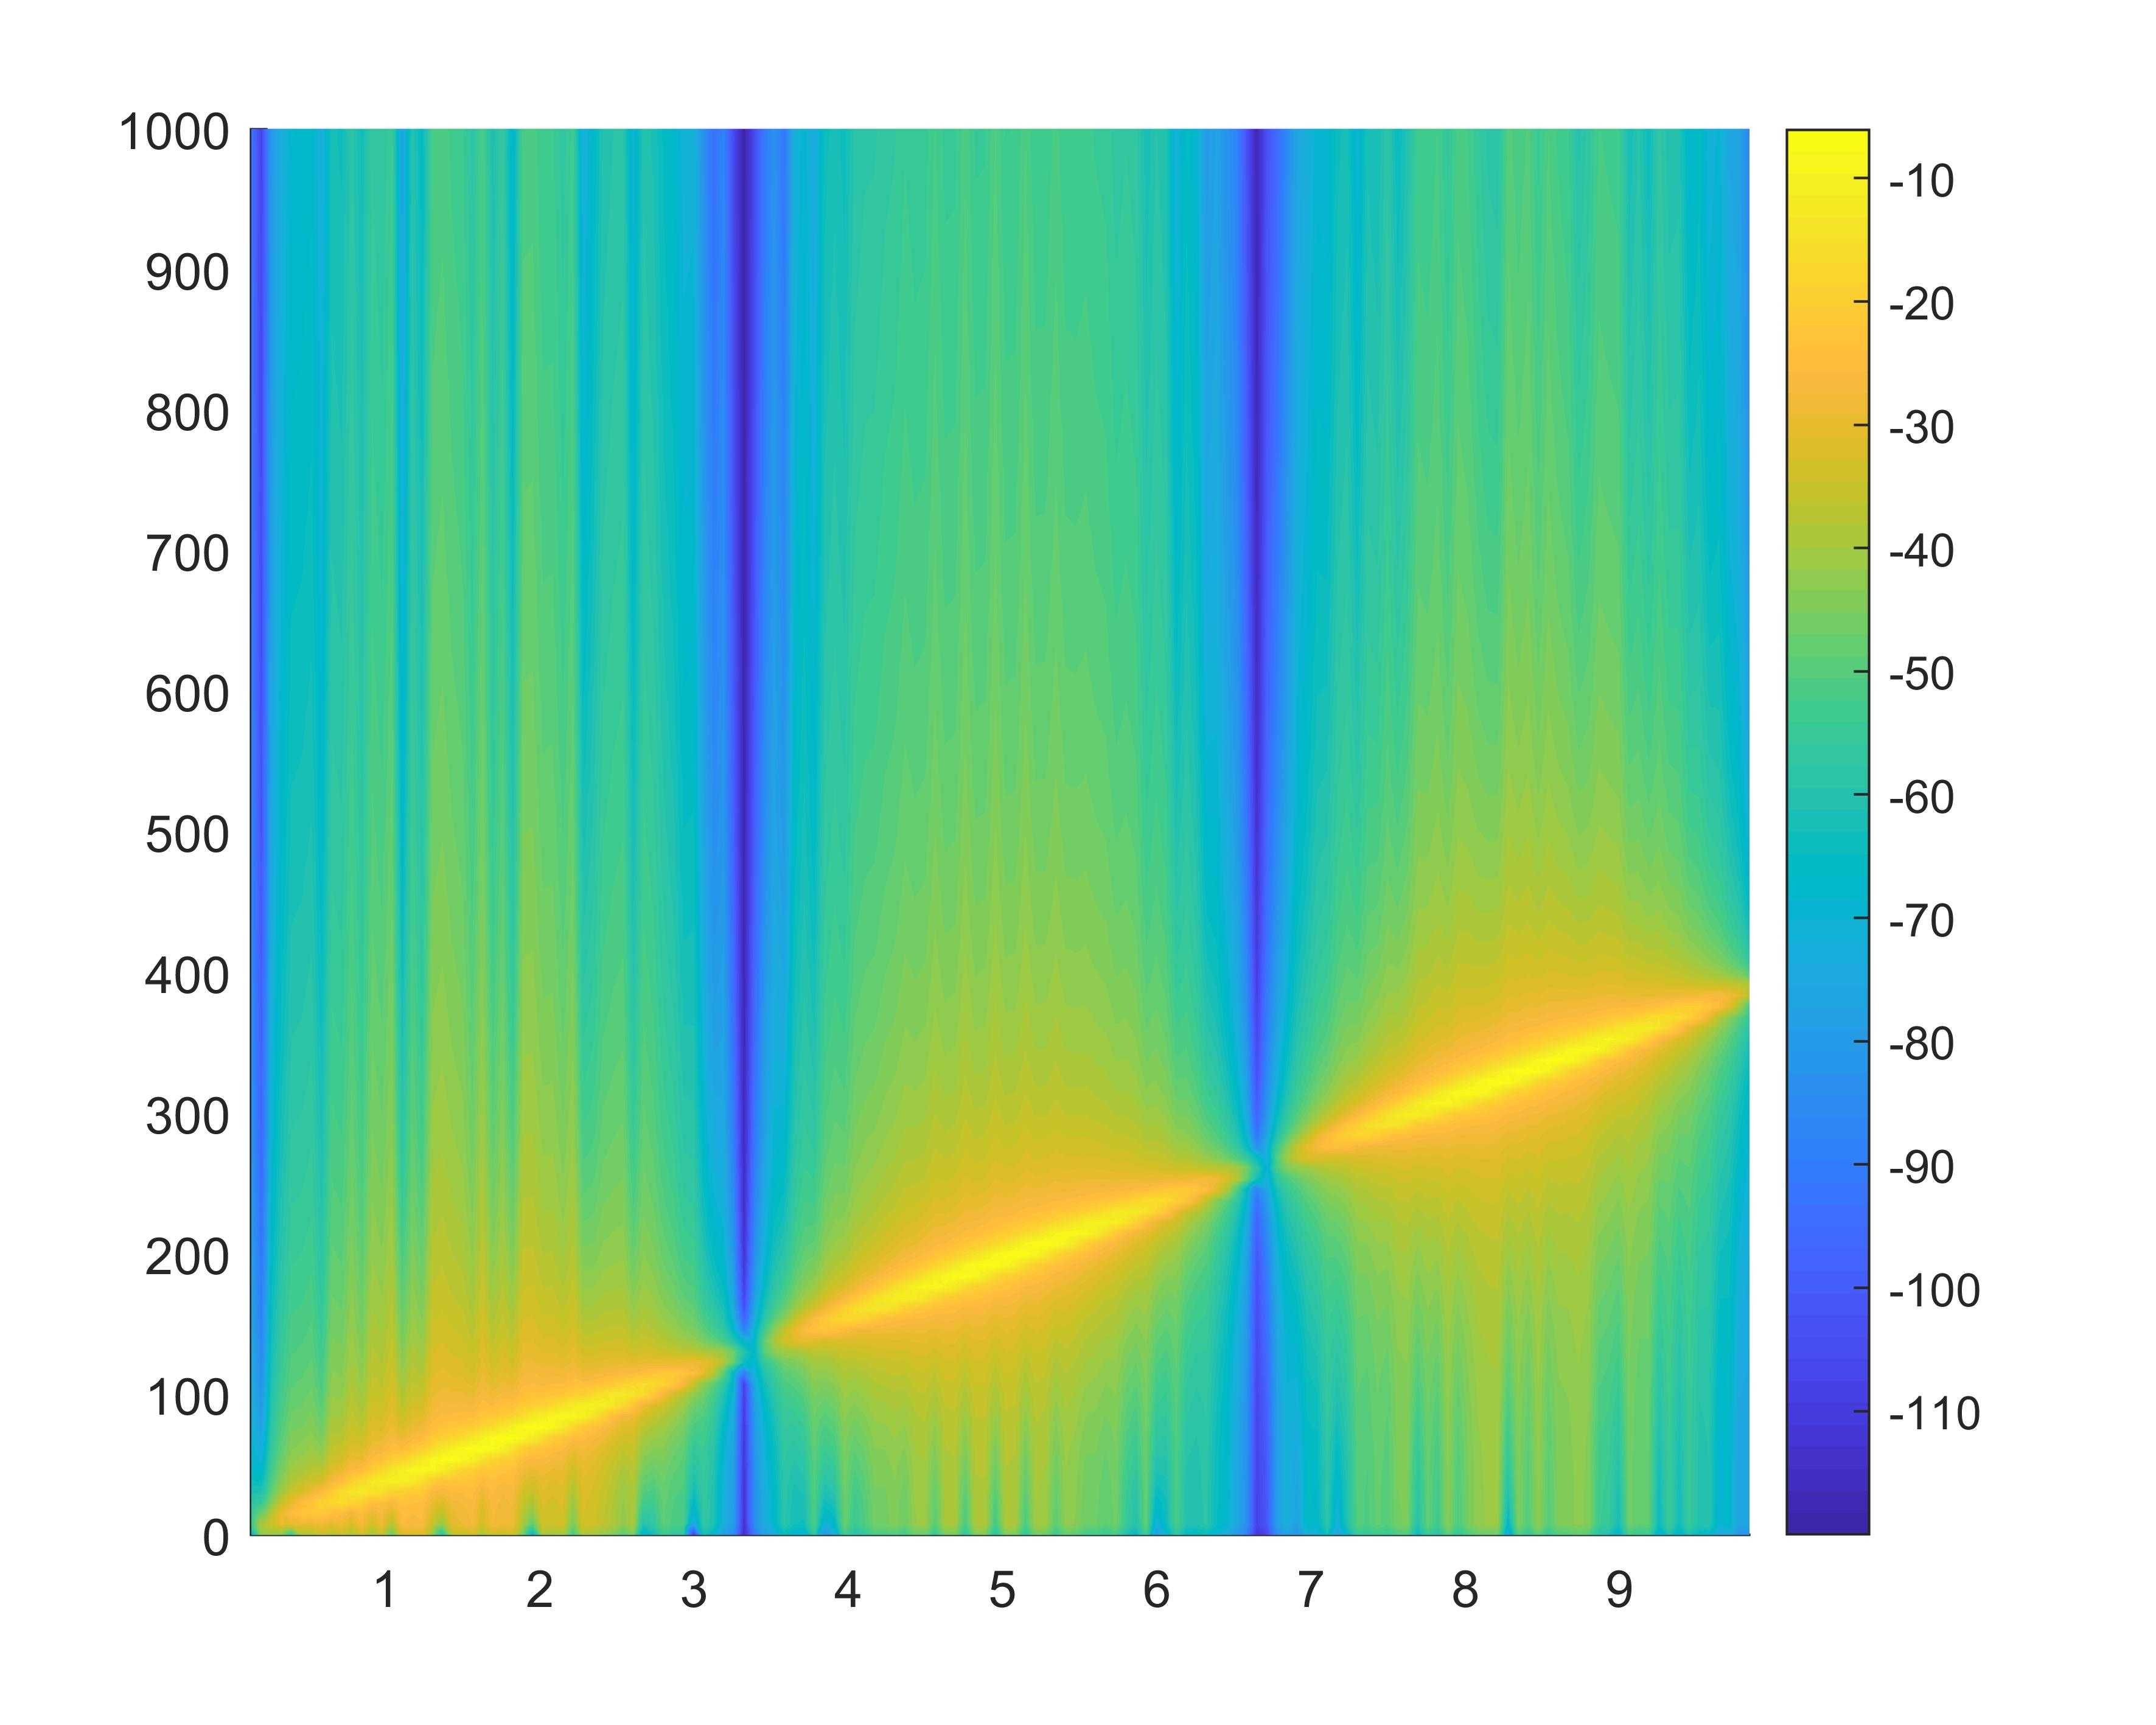
\includegraphics[width=\linewidth]{papers/autotune/sections/fft/stft8192.jpg}   
		\captionof{figure}{8192 Sample Fenster}\label{fig:stft8192}              \\           
	\end{tabularx}
	
	\caption{STFT}
	\label{fig:STFT}
\end{figure}%


Wie man bei der Abbildung \ref{fig:stft256} sieht, ist die Streuung ernorm. Mann kann nur sehr grob wahrnehmen, welche Frequenzen vorhanden sind, dafür ist die zeitliche Auflösung sehr gut. Die ist erkennbar an den scharfen Kanten an den Stellen wo das Testsignal eine Amplitude von Null hat. \\

Betrachtet man die Abbildung \ref{fig:stft1024} sind die Frequenzen schon viel deutlicher zu erkennen als bei einem Sampling von 256. Dafür wird in der zeitlichen Auflösung ein wenig eingebüsst.\\

Das beste Bild ist bei 4096 Samples in der Abbildung \ref{fig:stft4096} zu sehen. Die zeitliche Abgrenzung verschwimmt ein wenig. Dafür ist die Frequenz deutlich ersichtlich. Die Fensterlänge stellt rein zufällig den besten Kompromiss von Frequenz-Zeit-Auflösung dar.\\

In der letzten Abbildung \ref{fig:stft8192} ist die Zeit so langsam, dass die tiefen Frequenzen des Modultionssignal wieder Einfluss nehmen auf das Spektogramm. Dies verfälscht das Resultat. Ein solches Resultat kann bei praktischen Anwendungen weniger brauchbar sein, da eventuell die  langsame Modulationsfrequenz nicht so eine wichtige Rolle spielt. Anderseits könnte genau diese interessant sein weshalb die Fensterlänge nach Anwendung angepasst werden sollte.\\
\newpage





